% !TeX spellcheck = en_US
\addscenariosection{1}{Clash scenario}{Malwick Proposal!}{\images/morale_low.png}

\begin{multicols*}{2}

\textbf{Author:} Invoceusse

\textbf{Source:} \href{https://discord.com/channels/740870068178649108/1230205022705418302}{Archon Studio Discord}

\textit{During your hunt in Emerald island someone help you... But now it's time to pay your debt!\\
The only way for paying this? Thief one of your new friend, but you know that friend keep what you need in the center of this town : so you can only fight it for claim it!\\
Unfortunately your old friend cannot help you! He have the same mission, and only one of you can pay your debt!
}

\subsection*{\MakeUppercase{Scenario Length}}

This scenario is played over 13 rounds.

\subsection*{\MakeUppercase{Player setup}}

\textbf{Player Count:} 2 -- 3

\textbf{Starting Resources:}\par
\resources{15}{2}{0}

\textbf{Starting Income:}\par
\resources{10}{0}{1}

\textbf{Starting Units:}
\begin{itemize}
  \item A Few \svgunit{silver} units of your choice.
\end{itemize}

\textbf{Town Buildings:} \svgunit{bronze} Dwelling, City Hall.

\textbf{Map tile Pool:} None.

\textbf{Additional Bonus:} None.

\subsection*{\MakeUppercase{Map Setup}}

Take the following Map tiles and arrange them as shown in the scenario map layout ($P$ stands for the number of players):

$\boldsymbol{2 P}$ \textbf{× Starting (I) Map tile}
$\boldsymbol{2 P}$ \textbf{× Far (II--III) Map tile}
$\boldsymbol{4 P}$ \textbf{× Far (IV--V) Map tile}
$\boldsymbol{1 P}$ \textbf{× Far (VI--VII) Map tile}
\begin{itemize}
    \item All the I tiles next to VI-VII tile are AI towns.
    \item Some tile can't be rotated.
\end{itemize}

\subsection*{\MakeUppercase{Victory Conditions}}

First to flag your AI towns.\\
(However if a player kill their AI, finish the round! All player who have kill their AI the same round win.)

\subsection*{\MakeUppercase{Defeat Conditions}}

Lost battle again your AI.\\
A end of turn 13 if no one kill their AI, all players lose.

\subsection*{\MakeUppercase{Timed Events}}

\textbf{\nth{6} Round:}
\begin{itemize}
  \item Choose one field with a black cube you can reach, then gain again.
\end{itemize}
\textbf{end of \nth{12} Round:}
\begin{itemize}
    \item If you haven't reach your AI, immediately fight your AI but use turn 13 rule!
\end{itemize}

\subsection*{\MakeUppercase{Additional Rules}}
\begin{itemize}
    \item When a player go into one Tile I their is not this faction, gain 1 MP.
    \item Whenever a player visits an Obelisk, that player rolls one treasure dice and one resource dice, chooses one of the dice and resolves its outcome dice.
    \item After defeating a level VII neutral army, instead of resolving the tile, draw 4 cards from the spell deck and/or artifact deck and one from deck deck or artifact deck or ability deck, add the first card of the spell/ability/artifact discard, you can add up to 2 of these 8 cards and gain 12 gold.
    \item If you failed battle, even if all your unit are killed, move your hero back to the field they last visited (and not in your town).
    \item Additionally, no player can go to other player town (but can go into AI town).
\end{itemize}

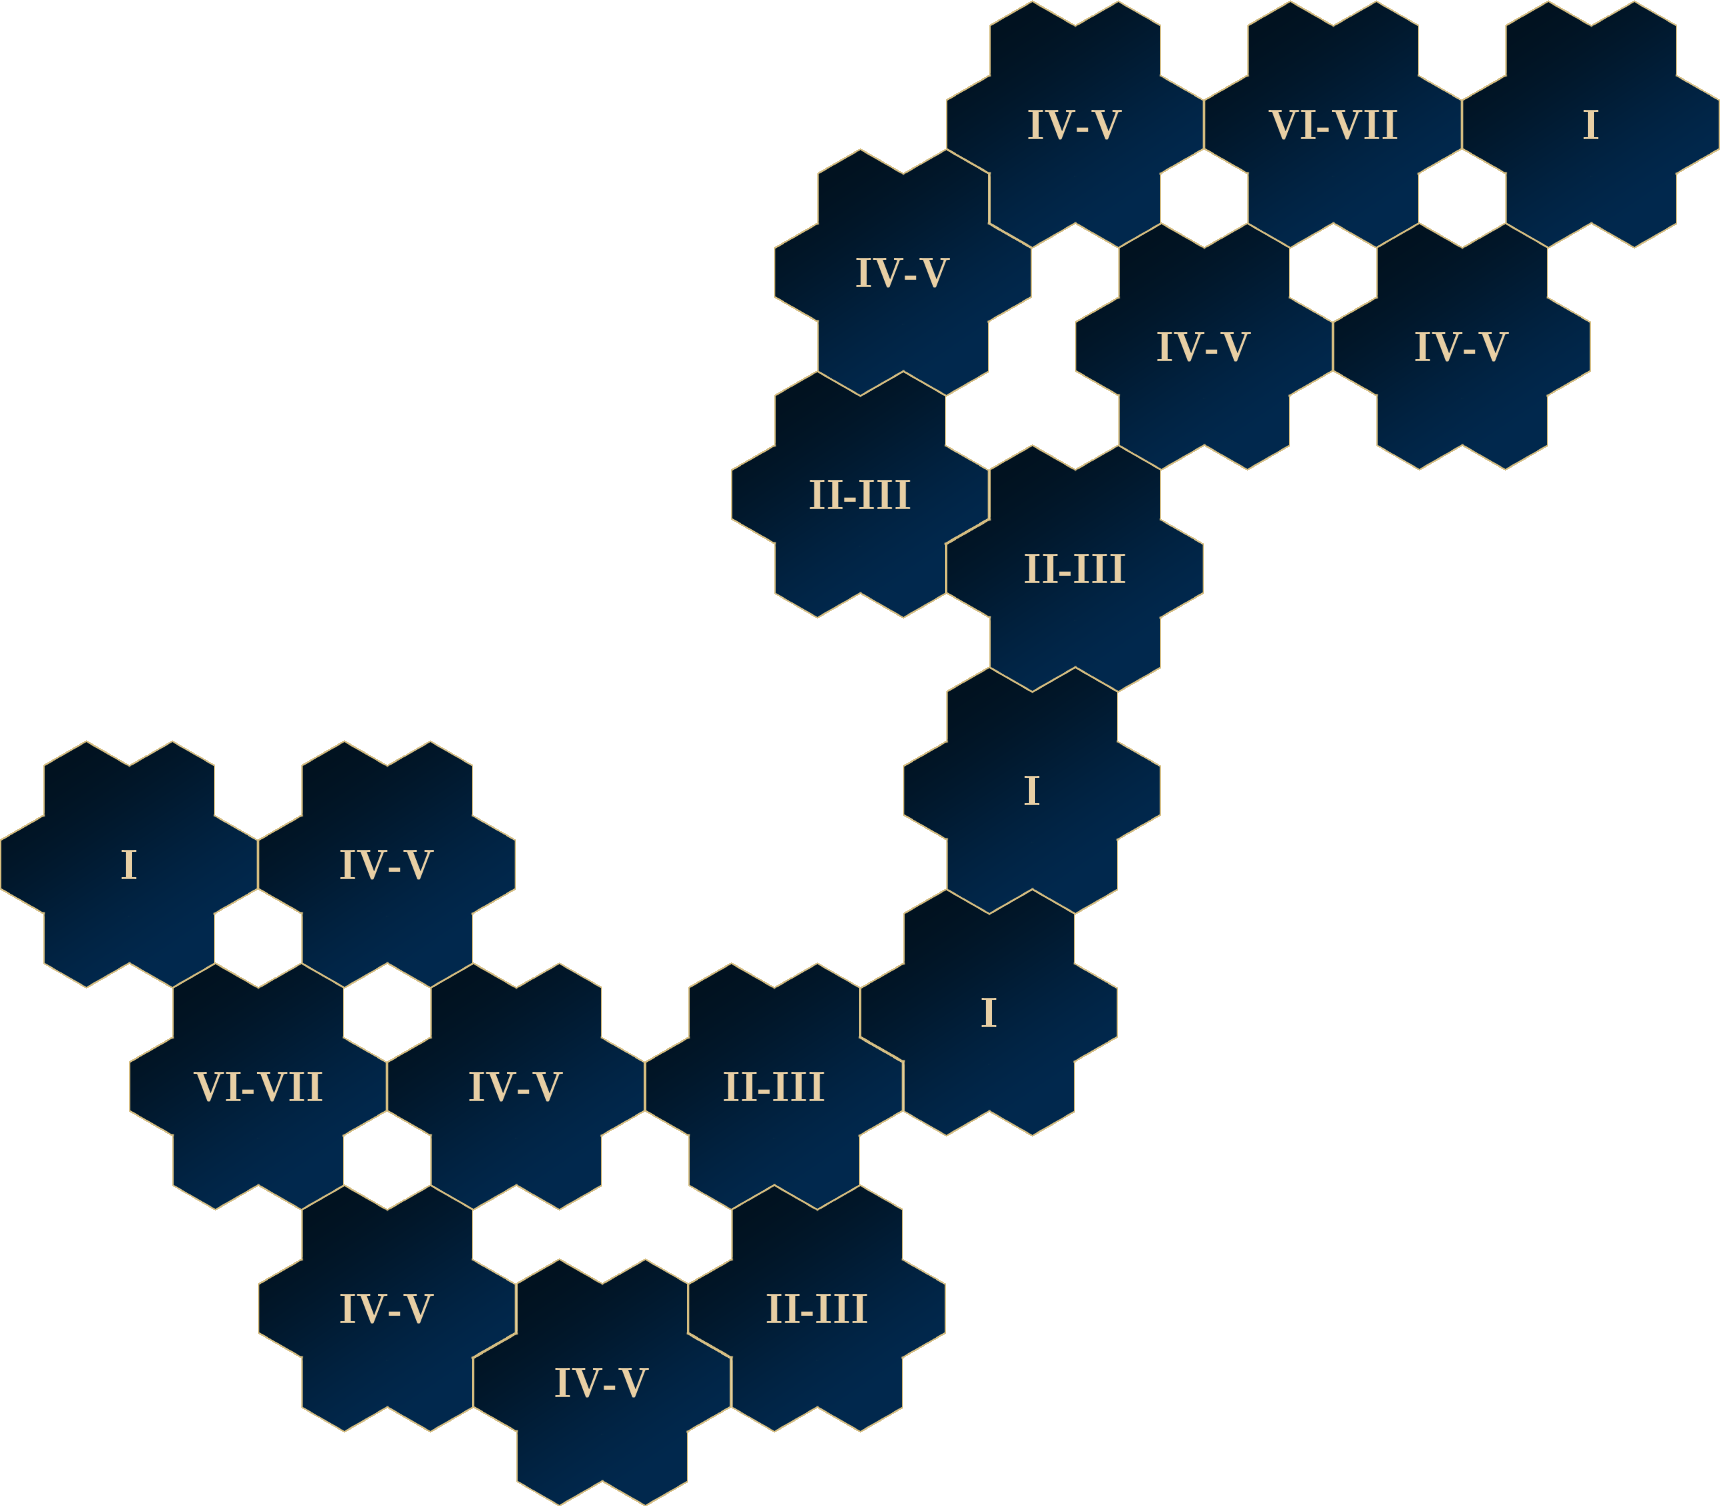
\includegraphics[width=0.6\paperwidth]{\_assets/maps/malwick_dark_2.png}
\captionof{figure}{2-PLAYER SCENARIO}
\vspace{3em}

\end{multicols*}

\begin{center}
    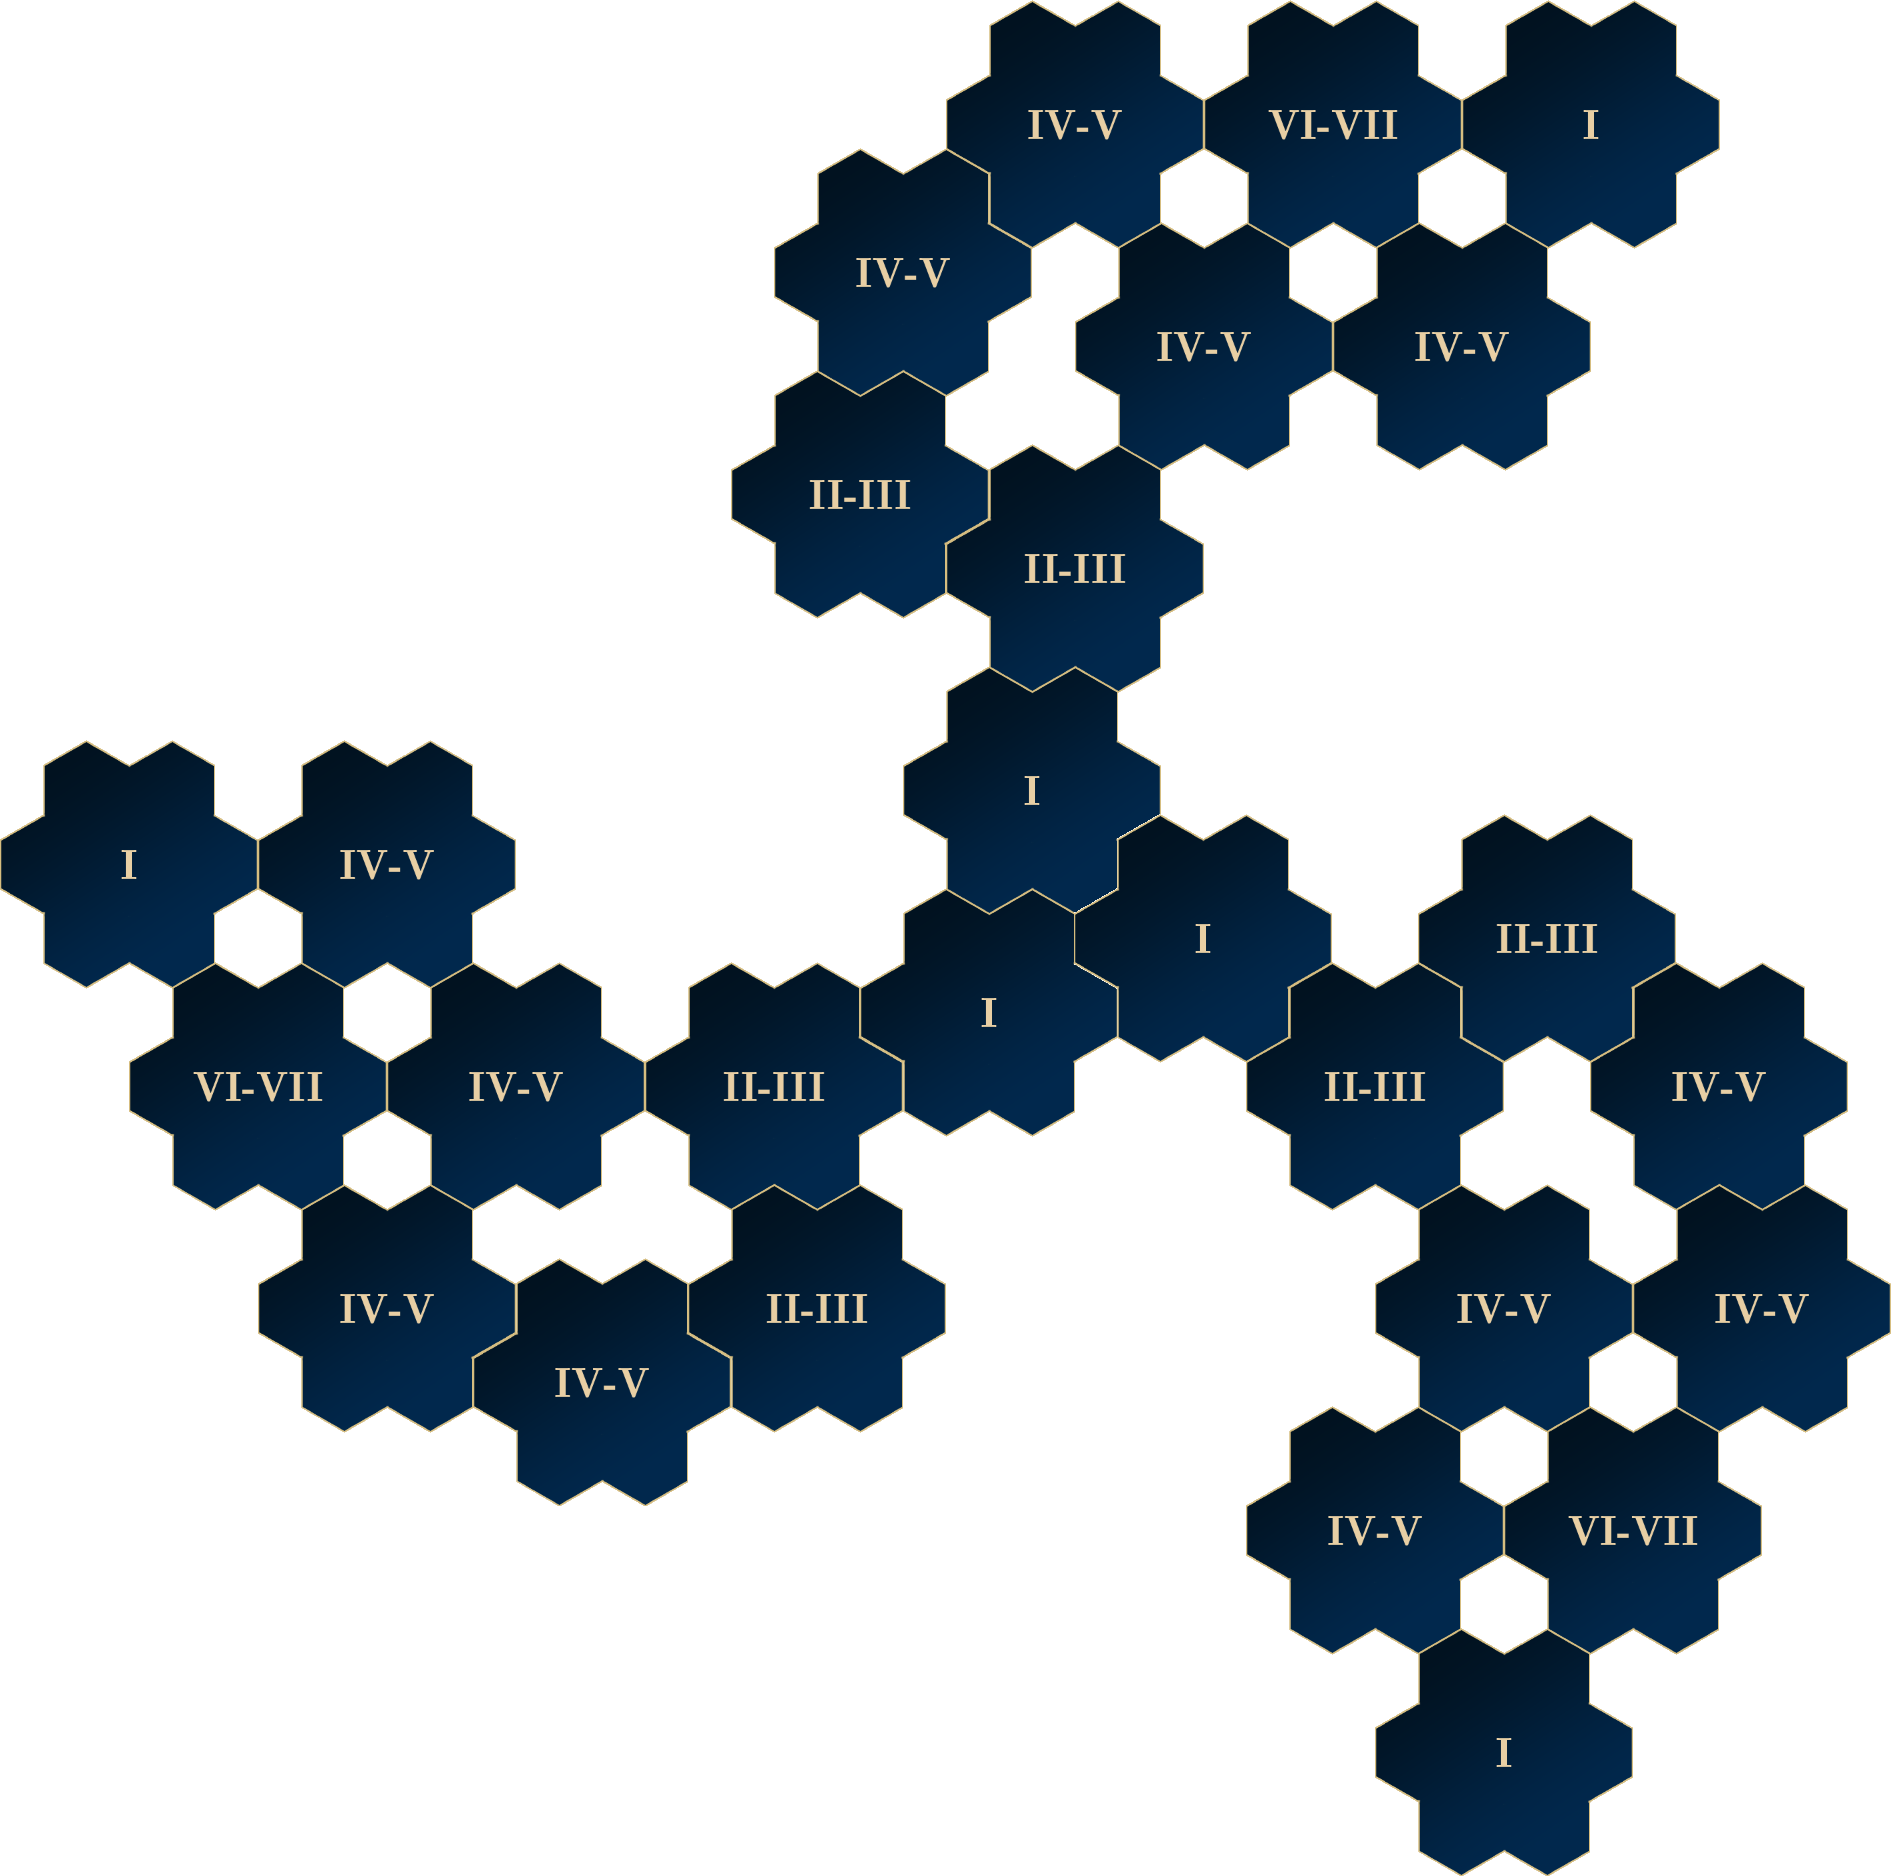
\includegraphics[width=0.8\paperwidth]{\_assets/maps/malwick_dark_3.png}
    \captionof{figure}{3-PLAYER SCENARIO}
\end{center}
